\chapter{Circuit output measurement results in time domain}
\textit{The heart of the thesis, comprising a presentation of the functioning system and thus the culmination of the work. Important is an analysis of the results as well as a comparison with the state of the art. The reader should understand in this section why you should be awarded a MSc degree.}

To demonstrate that the designed circuits really can synthesize a signal from a digital input signal, a time domain measurement would be necessary.
To measure in time domain, an oscilloscope comes to mind.
An important aspect is that the output impedance in chapter \ref{ch:design} is calculated but not assembled. 
The concept is based on the fact, that this circuit is pumping charges onto a output capacitance.
This output capacitance should be the input of a power amplifier as a GAN transistor.
Due to the fact that no power amplifier is connected to the output, the question comes to mind how to measure the output if no capacitance is connected to it with the oscilloscope.
A first try is to show the push-pull of the supply voltage. 
This only would demonstrate the one bit switching but it would show that if a one bit switch is functioning properly, two or three bit are not as far as assumed.
The second try would be to connect it to an active load pull measurement, but here the drawback is the limited harmonic control and that the input signal is limited in frequency and steepnes. 
As we want to digital control the circuit, a rectangular signal is needed.
As we want a signal frequency of 100 MHz, an input frequency of at least 800 MHz is required.\\

\section{Measurement setup}
Here an overview of the measurement setup is given. 


\begin{figure}[htb!]
	\centering
  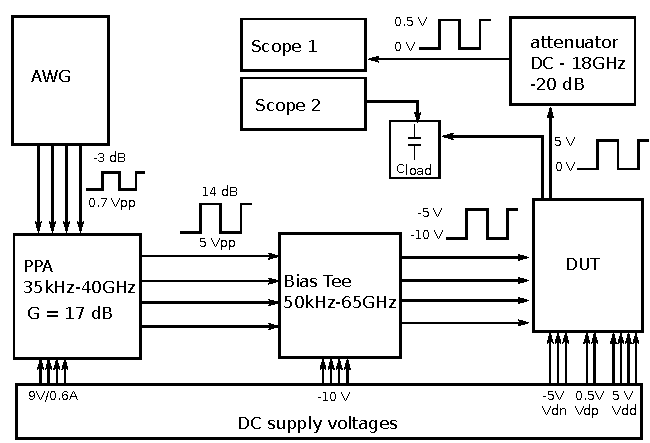
\includegraphics{MeasurementSetup.pdf}
	\caption{Schematic of broadband time domain measurement setup}
	\label{fig:SchematicMeasSetup}
\end{figure}



The \gls{ab:dc} supply is the same for both measurement setups.
The input control is depending on the system which is used for the measurement.\\
First option would be to scope a real time output (on-wafer) with an oscilloscope.
For the output signal measurement in time domain with the oscilloscope the digital input signal is delivered from a high speed AWG.
The digital input is generated from the AWG, amplified by an preamplifier to get a voltage swing of 5Vpp and at last a dc bias tee is connected to ensure the correct dc offset to the input.
 The input is controlled by an AWG from Keysight, programmed with a determined data set of bits. The key components are listed here:
\begin{itemize}
	\item Keysight AWG - (1V := 0dB; 0.7V := -3dB)
	\item Broadband (35kHz-40GHz) amplifier (17dB gain) (digital signal with clk 1GHz, 10 harmonics -> 10GHz)
	\item Bias Tees (DC bias)
	\item DC supply (driver network, power transistor)
	\item DUT
	\item LOAD - OUTPUT ???
\end{itemize}

Secondly the output measurement with (anteverta) active load pull system is done.
For this measurement no AWG is needed to provide the digital input signal, since the measurement is done with a Anteverta active load pull system, this device is providing the input signal.
In fact of knowing its input and output signal this device is capable to tune the impedance at arbitrary points in the circuit.
This is a nice way to simulate a capacitive load at the output to show the behaviour of the circuit with this load impedance calculated in \ref{ch:design}.
By using this active load pull system, we have to reduce the number of bits for the resolution to one bit due to the fact, that the system only provide the option to handle four harmonics. 
We already use two harmonics for the differential input signal and one harmonic for the output tuning the impedance. 
Hence there is only one harmonic left for which no other input can controlled since two signals are necessary to get a differential input signal.
\section{Time domain measurement}
\begin{enumerate}
	\item calibration measurement instruments
	\item DC supply check - whether oscillates or not
	\item Output measurement for switching 1-bit
	\item \textit{passive cap at the load to show the concurrent switching of both bits}
	\item \textit{anteverta system to realize a capacitive load impedance}
\end{enumerate}



\begin{figure}[htb!]
	\centering
  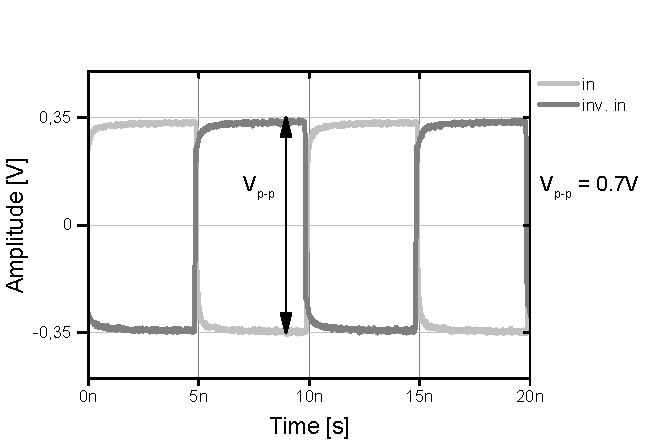
\includegraphics{inputVoltage.pdf}
	\caption{time domain measurement input control voltage}
	\label{fig:inputMeas}
\end{figure}

\begin{figure}[htb!]
	\centering
  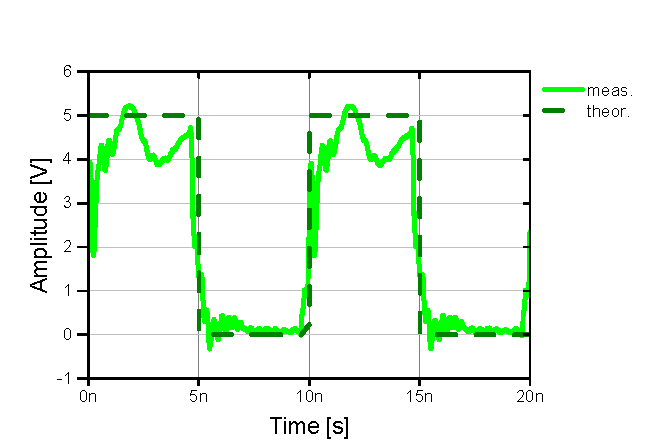
\includegraphics{100M_Rload_regression.pdf}
	\caption{time domain measurement of output voltage with 50 Ohm termination}
	\label{fig:measRload100M}
\end{figure}



\begin{figure}[htb!]
	\centering
  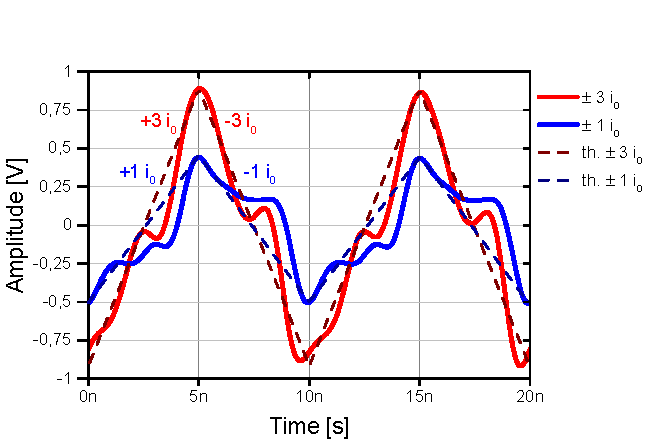
\includegraphics{100M_Cload_regression.pdf}
	\caption{time domain measurement with capacitive load}
	\label{fig:measCload100M}
\end{figure}

\begin{figure}[htb!]
	\centering
  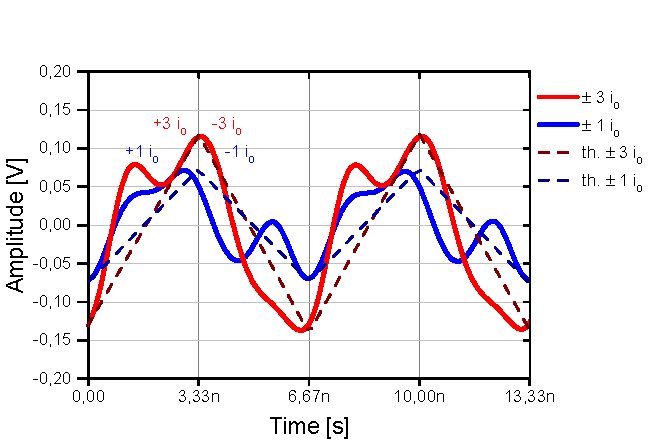
\includegraphics{150M_Cload_regression.pdf}
	\caption{time domain measurement with capacitive load}
	\label{fig:measCload150M}
\end{figure}

Load capacitance is 3n3F.

\section{Discussion of measurement results}
In a first step it is to show that the designed circuit converts a digital signal to an analog one. It would be nice to see any effect corresponding to the digital to analogue conversion. \\
\textit{is it possible to measure the heat spreading on the substrate?}
Is the measurement result expected due to the simulation? Can the demonstrator be simulated although no model for this chips exists? The real simulation are not done due to the fact that no losses respected.

